\documentclass[12pt]{article}

\usepackage{sbc2003}

\usepackage{graphicx,url}

\usepackage[brazil]{babel}   
\usepackage[utf8]{inputenc}

% Para estilização dos códigos
\usepackage{minted}

% Para lista em linhas
\usepackage{paralist}

% Identar primeiros parágrafos
\usepackage{indentfirst}

%TODO
\usepackage[colorinlistoftodos]{todonotes}

\usepackage{minted}

\usepackage{array}

%---
% Pacote para listas em uma linha
%---
\usepackage{paralist}

\title{Colagem, recorte e erros em um processo composicional utilizando o Music21.}

\author{Guilherme Lunhani\inst{1}}

\address{Instituto de Artes e Design --
         Universidade Federal de Juiz de Fora \\
         Juiz de Fora, MG
         \email{gcravista@gmail.com}
}

\begin{document}

\maketitle

\begin{abstract}
This article describes a case study in Computer Generated Assistance, for music analysis and didactic composition. A Python command was programmed to automate routines based on \cite{music21_2015} library, such: selection, cluster and fragmentation from a document in J.S.Bach's corpus. Some compositional exercises were used to test a operation, called \emph{glitch}, in this corpus. In addition, \cite{musescore_2015} and \cite{lilypond_2015} were used to edit and diagram scores. At the end, comment on bugs, compositional problems and future plans of composition.
\end{abstract}

\begin{resumo}
Este artigo descreve um estudo de caso em Assitência Gerada por Computador para análise musical e composição didática. Um comando {Python} foi programado para automatizar rotinas da biblioteca \cite{music21_2015} como: seleção, agrupamento e fragmentação de um documento no corpus bachiano. Alguns exercícios composicionais foram usados para testar uma operação \emph{glitch}, neste corpus. Adicionalmente,  \cite{musescore_2015} e \cite{lilypond_2015} foram utilizados para edição. Ao final comentarei \emph{bugs}, problemas composicionais  e planos futuros de composição.
\end{resumo}

\section{Introdução}

Este artigo trata de um protótipo de ferramenta, \emph{m21.py}, um binário \emph{Python} para manipulação criativa e analítica do \cite{music21_2015}. Na seção \ref{sec:trabalhos}, relacionamos alguns textos à elaboração do programa. Na seção \ref{sec:justificativa} uma justificativa para o projeto. 

Uma descrição dos métodos de desenvolvimento, e do método criativo (aplicado aos materiais pré-composicionais gerados), são explicados na seção \ref{sec:metodo}. Na seção \ref{sec:m21} são apresentados alguns detalhes da ferramenta, úteis no processo de geração do material. Na seção \ref{sec:resultados}, é apresentado um exemplo prático. 

Na seção \ref{sec:conclusao} são apresentados problemas técnicos observados, e uma autocrítica. Na seção \ref{sec:planos}, os planos futuros de desenvolvimento.
\section{Trabalhos relacionados}\label{sec:trabalhos}

Durante uma pesquisa de mestrado, sobre \emph{live coding}, tive contato com o Music21 que, segundo \cite{soares_luteria_2015}:

\begin{quote}
É uma biblioteca projetada para trabalhar com manipulação e análise de corpus de arquivos partituráveis. Prepara a conversão entre diversos arquivos de dados musicais. (\ldots) Music21 tem uma abordagem voltada para uma "musicologia assistida por computador" e já tem incorporada em suas classes algumas ferramentas comuns a esta prática como: numeração de grau funcional de acorde, numeração de classes de altura usando a classificação de Allen Forte : a implementação dos algoritmos de detecção de tonalidade elaborado por Krumhansl (1990) e aperfeiçoada por Temperley (2001), busca de padrões como transposições e inversões e outros.\cite[p.~71-72]{soares_luteria_2015}
\end{quote}

Ao invés de compor adicionando informações aos dados musicais, busquei na \emph{Estética do Erro} \cite{cascone_aesthetics_2000} os procedimentos básicos para composição, explicados com mais detalhes na seção \ref{sec:metodo}. Resultados sonoros procedentes da colagem e do erro dependem muito do \emph{input}. Aplicar o mesmo algoritmo de erro para diferentes materiais, ou, aplicar diferentes erros para um único material, não resulta em um produto homogêneo.

Busquei então utilizar diferentes documentos do \emph{corpus}, e um mesmo erro para realizar um tipo de música que, segundo \cite[p.~18]{soares_luteria_2015}, existia intensamente ``antes da preocupação imediata com os timbres ou da era das manipulações de amostras sonoras - e de certa maneira ainda proto-serialista. Uma música por vezes chamada politonal, polimodal ou usando o termo de Straus (2004): pós-tonal.''. Sendo um tipo de composição que não é nova, mas relevante do ponto de vista histórico e didático-composicional,  busquei elaborar uma ferramenta para ser usada em processos criativos musicais. 

\subsection*{Questões pessoais}

Não deixo de mencionar uma antiga conversa com o compositor Franscisco Zmekhol Nascimento de Oliveira, que levou-me a compor segundo regras arbitrárias, na contingência do momento. Isto é, uma música para cada dia da existência. 

Ao realizar o mesmo procedimento de composição de um mesmo documento do \emph{corpus} bachiano, o material pré-composicional resultante deve ser diferente de qualquer outro. 

Para realizar tecnicamente, valores não-determinados em operações determinísticas são utilizados.

Para compor-improvisar com os materiais resultantes, apliquei princípios de articulação do som pelo silêncio, elaborados por rascunhos de partituras-planimétricas, utilizadas por \cite{koellreutter_introducao_1987}.
\section{Metodologia}\label{sec:metodo}

\subsection*{Organização dos códigos}

O programa foi separado em três arquivos: \begin{inparaenum}[\itshape i)\upshape]
\item um binário em \emph{Python} que realiza tarefas gerais da linha de comando (\emph{m21});
\item rotinas do Music21 (\emph{m21utils.py}); e 
\item um para rotinas externas (\emph{tools.py})
\end{inparaenum}\footnote{Todos códigos, exemplos e documentação estão disponíveis \url{https://www.github.com/jahpd/m21}.}.

\subsection*{Categorização do software}

Nas palavras de \cite[p.~x-xiii]{cope_prefacio_2008}, o \emph{m21} pode ser classificado como uma ferramenta para uma Assistência Gerada por Computador (\emph{Computer Generated Assistance} ou CGA). Dentro das sub-categorias de CGA propostas por Cope, o \emph{m21} pode ser incuído nos três modos abaixo:\begin{inparaenum}[\itshape 1)\upshape]
\item uso de uma Linguagem de Programação em texto (PLs)(\emph{Programming Languages}) ao invés de uma linguagem de programação visual (VPL); 
\item o material partitural é gerado para performance humana ao invés de uma performance eletroacústica;
\item abordagens baseadas em regras (\emph{Rules Based}) e Dirigido a dado (\emph{Data-Driven}) são usados para modificar um material existente.
\end{inparaenum}

\subsection*{Método de composição}

Em geral, o procedimento de composição se deu a partir da execução de um comando \emph{m21} com argumentos explicados na seção \ref{sec:resultados}: \begin{inparaenum}[\itshape i)\upshape]
\item gerar um material musical com base em uma colagem de uma obra no corpus do Music21;
\item o material colado será submetido a subtração de compassos, aleatoriamente;
\item dos compassos restantes, quaisquer notas serão agrupadas como um evento;
\item destes agrupamentos, as oitavas serão embaralhadas; e
\item do bloco harmônico resultante, pode ser que alguma nota fique deslocada, gerando figuras.
\end{inparaenum}

Busquei notar densidades, fraseado e pontos de finalização ``naturais'' do material harmônico resultante Tais parâmetros eram editados no MuseScore, sendo que algumas interferências não previstas foram incluídas. Após edição, ocorreu o processo de editoração no Lilypound para melhor visualização dos resultados.

Por último, o material pré-composicional foi editado no \cite{musescore_2015} e posteriorente diagramado no \cite{lilypond_2015}.
\section{M21}\label{sec:m21}

\subsection{Instalação e uso}

\subsubsection*{Pelo terminal}
Considerando que o sistema operacional já possui o \emph{git}\footnote{https://en.wikipedia.com/git}, podem ser dados os seguintes comando em um terminal.

\begin{minted}[linenos,frame=leftline,fontsize=\footnotesize]{python}
guilherme@R410-L-BP12P1 > git clone https://www.github.com/jahpd/m21.git
guilherme@R410-L-BP12P1 > cd m21
guilherme@R410-L-BP12P1 > chmod u+x ./m21
\end{minted}

\subsubsection*{Opções}

Ao executar o comando $help$ é obtida uma página de ajuda.

\begin{minted}[linenos,frame=leftline,fontsize=\scriptsize]{python}
guilherme@R410-L-BP12P1 > ./m21 --help
Usage: m21 [OPTIONS, [ARGS]]

For computer assisted musicology and composition

Options:
  --version             show program's version number and exit
  -h, --help            show this help message and exit
  -s, --search-only     Search in corpus for words in --composer and or
                        --index arguments. Ex.: --composer bach --index bwv1x
  -c COMPOSER, --composer=COMPOSER
                        write report with specific corpora. CAUTION: you must
                        use this according http://web.mit.edu/music21/doc/syst
                        emReference/referenceCorpus.html#referencecorpus
  -i INDEX, --index=INDEX
                        Search in corpus specific index of corpora; you must
                        use this with -c option, according available corpora
                        in  http://web.mit.edu/music21/doc/systemReference/ref
                        erenceCorpus.html#referencecorpus
  -C, --CAC             Or simple "Computer Assisted Composition". With this
                        option you will "glitch" a specific piece, as
                        instance, with --composer/--index options, --xml
                        option or --tiny-notation option. Adding --fragmentize
                        option with a value (ex: --fragmentize 4, max 6), you
                        will apply a "fragmentation" on input. You can add
                        --no-scramble-notes, --no-scramble-octaves and
                        arguments.
  -n, --no-scramble-notes
                        with this option, the program will not apply a
                        scramble on list of extracted notes, before create
                        chords
  -N, --no-scramble-octaves
                        With this option, the program will not apply a
                        scramble on list of extracted octaves, before create
                        chords
  -g GLITCH, --glitch=GLITCH
                        Apply a'glitch' on extracted notes and octaves; the
                        given argument is the maximum of a random operation.
                        This operation can be a choice of a 6 values: (0) The
                        generated chord will be arranged in closed position;
                        (1) the generated chord will be arranged in semi-
                        closed position; (2) the generated chord will be
                        arranged in super open position; (3) one note will be
                        separated from chord, like an one grace note; (4) two
                        notes will be separated from chord (if this chord have
                        at least, two notes); (5) apply bordadure [? translate
                        ?], and then a chord
  -m MEASURES, --measures=MEASURES
                        Select measures from a stream (corpus, xml or
                        tinynotation)
  -R, --reducte         Reducte some stream to piano staff
  -A TONAL_HARMONIC_ANALYSIS, --tonal-harmonic-analysis=TONAL_HARMONIC_ANALYSIS
                        Analyse some stream in tonal way, given some key
  -S, --show            show stream in some editor (musescore default)
  -x XML, --xml=XML     parse a musicXml file; can be a local one or http url
  -t TINYNOTATION, --tinynotation=TINYNOTATION
                        parse a tiny-notation (ex: --tiny-notation "2/16 E4 r
                        f# g=lastG trip{b-8 a g} c".
  -T TITLE, --title=TITLE
                        used to give a title. (ex: --title "My improvised
                        music"
  -a AUTHOR, --author=AUTHOR
                        used to give a author. (ex: --author "J.S. Bach"
  -r TRANSPOSE, --transpose=TRANSPOSE
                        transpose stream notes by semitones (ex.: --transpose
                        4 will transpose to a ascendent major third and
                        --transpose -4 will transpose to a descendent major
                        third
  -I, --invert          invert stream intervals by semitones. No need
                        arguments
  -L LYTEXIFY, --lytexify=LYTEXIFY
                        Create a .lytex file from a .ly file, and compiles it
                        to a .tex file. Used only in the context of
                        documentation of this software
  --plot-stream         analysis graph with PlotStream class
  --plot-histogram-pitch-space
                        analysis graph with PlotHistogramPitchSpace class
  --plot-histogram-pitch-class
                        analysis graph with PlotHistogramPitchClass class
  --plot-histogram-quarter-length
                        analysis graph with PlotHistogramQuarterLength class
  --plot-scatter-pitch-space-quarter-length
                        analysis graph with PlotScatterPitchSpaceQuarterLength
                        class
  --plot-scatter-pitch-class-quarter-length
                        analysis graph with PlotScatterPitchClassQuarterLength
                        class
  --plot-scatter-pitch-class-offset
                        analysis graph with PlotScatterPitchClassOffset class
  --plot-scatter-pitch-space-dynamic-symbol
                        analysis graph with PlotScatterPitchSpaceDynamicSymbol
                        class
  --plot-horizontal-bar-pitch-space-offset
                        analysis graph with PlotHorizontalBarPitchSpaceOffset
                        class
  --plot-horizontal-bar-pitch-class-offset
                        analysis graph with PlotHorizontalBarPitchClassOffset
                        class
  --plot-scatter-weighted-pitch-space-quarter-length
                        analysis graph with
                        PlotScatterWeightedPitchSpaceQuarterLength class
  --plot-scatter-weighted-pitch-class-quarter-length
                        analysis graph with
                        PlotScatterWeightedPitchClassQuarterLength class
  --plot-scatter-weighted-pitch-space-dynamic-symbol
                        analysis graph with
                        PlotScatterWeightedPitchSpaceDynamicSymbol class
  --plot3-d-bars-pitch-space-quarter-length
                        analysis graph with Plot3DBarsPitchSpaceQuarterLength
                        class
  --plot-windowed-krumhansl-schmuckler
                        analysis graph with PlotWindowedKrumhanslSchmuckler
                        class
  --plot-windowed-krumhansl-kesslerm
                        analysis graph with PlotWindowedKrumhanslKesslerm
                        class
  --plot-windowed-aarden-essen
                        analysis graph with PlotWindowedAardenEssen class
  --plot-windowed-simple-weights
                        analysis graph with PlotWindowedSimpleWeights class
  --plot-windowed-bellman-budge
                        analysis graph with PlotWindowedBellmanBudge class
  --plot-windowed-temperley-kostka-payne
                        analysis graph with PlotWindowedTemperleyKostkaPayne
                        class
  --plot-windowed-ambitus
                        analysis graph with PlotWindowedAmbitus class
  --plot-dolan          analysis graph with PlotDolan class
\end{minted}

\subsubsection*{Alguns usos básicos}

Os comandos podem ter sua forma longa e curta; por exemplo \verb|--composer| pode ser abreviado para \verb|-c|. Abaixo listamos alguns dos mais usados durante o trabalho

\subsubsection*{Procurar por compositores ou obras  no \emph{corpus}}:
\begin{minted}[linenos,frame=leftline,fontsize=\footnotesize]{python}
./m21 --search-only --composer bach
./m21 -s -c bach -i bwv1
./m21 --search-only --index bwv1
./m21 -s -i bwv1
\end{minted}

\subsubsection*{Mostrar em um \emph{software} de editoração musical uma obra do \emph{corpus}.}

De acordo com a documentação oficial, um \emph{software} externo pode ser usado para abrir aquivos formatados em \emph{musicXml}. Como é um formato padrão, diferentes editores de partitura podem ser usados. Entre eles Finale e Sibelius. Neste artigo utilizamos o \cite{musescore_2015}. Para alterar qual deles será usado, é necessário modificar a variável \verb|musicxmlPath| no arquivo \verb|~/.music21.rc| (em sistemas Unix), criado durante a instalação.

\begin{minted}[linenos,frame=leftline,fontsize=\footnotesize]{python}
./m21 --show --composer bach --index bwv1
./m21 -S -c bach -i bwv1
\end{minted}

\subsubsection*{Mostrar no Musescore um arquivo do tipo musicxml.}

\begin{minted}[linenos,frame=leftline,fontsize=\footnotesize]{python}
./m21 --show --xml bwv1.xml
./m21 -S -x bwv1.xml
\end{minted}

\subsubsection*{Mostrar no Musescore uma idéia musical improvisada.}

É possível escrever rapidamente uma idéia musical. Um pequeno exemplo de codificação foi realizado abaixo com um motivo da primeira invenção de Bach.

\begin{minted}[linenos,frame=leftline,fontsize=\footnotesize]{python}
./m21 -show --tinynotation "2/4 r16 c d e f d e c g8 c' b c' d'"
./m21 -S -t "2/4 r16 c d e f d e c g8 c' b c' d'"
\end{minted}

\begin{figure}[h]
  \centering
  {%
\parindent 0pt
\noindent
\ifx\preLilyPondExample \undefined
\else
  \expandafter\preLilyPondExample
\fi
\def\lilypondbook{}%

\includegraphics{../examples/tinynotation/42/lily-08b23daa-1}%
\ifx\betweenLilyPondSystem \undefined
  \linebreak
\else
  \expandafter\betweenLilyPondSystem{1}%
\fi

\includegraphics{../examples/tinynotation/42/lily-08b23daa-2}%
% eof

\ifx\postLilyPondExample \undefined
\else
  \expandafter\postLilyPondExample
\fi
}

  \caption{Motivo principal da invenção em dó maior J.S. Bach, BWV X, escrito rapidamente n terminal. Metadados necessitam de correções \textbf{Fonte}: autor}
    \label{fig:tinynotation}
\end{figure}

\subsubsection*{Mostrar no Musescore um recorte de uma obra no \emph{corpus}.}

Apresentar um fragmento de uma peça. Abaixo recortei os cinco primeiros compassos do BWV1, como na figura \ref{fig:bwv_frag}:

\begin{minted}[linenos,frame=leftline,fontsize=\footnotesize]{python}
./m21 --show --composer bach --index bwv1 --measures 0 4
./m21 -S -c bach -i bwv1 -m 0 4
\end{minted}

\begin{figure}[h]
  \centering
  {%
\parindent 0pt
\noindent
\ifx\preLilyPondExample \undefined
\else
  \expandafter\preLilyPondExample
\fi
\def\lilypondbook{}%

\includegraphics{../analysis/bwv1/2a/lily-0aa3d7a2-1}%
\ifx\betweenLilyPondSystem \undefined
  \linebreak
\else
  \expandafter\betweenLilyPondSystem{1}%
\fi

\includegraphics{../analysis/bwv1/2a/lily-0aa3d7a2-2}%
\ifx\betweenLilyPondSystem \undefined
  \linebreak
\else
  \expandafter\betweenLilyPondSystem{2}%
\fi

\includegraphics{../analysis/bwv1/2a/lily-0aa3d7a2-3}%
% eof

\ifx\postLilyPondExample \undefined
\else
  \expandafter\postLilyPondExample
\fi
}

  \caption{Extração dos cinco primeiros compassos (\emph{measures}) do BWV1.6, utilizando o comando \emph{./m21 -c bach -i bwv1 -m 0 4}}
    \label{fig:bwv_frag}
\end{figure}

\subsubsection*{Analisar uma peça tonal} 

Por exemplo, os cinco primeiros compassos anteriores (quatro compassos e anacruse) podem ser analisados em qualquer tom. Considerando que o grau I é Fá, indicamos na linha de comando a representação alfabética, ou a letra \textbf{F} será apresentado o resultado como na figura \ref{fig:bwv_anal}. Qualquer outra nota utilizada para análise irá gerar um ``processo proporcional'', mas incorreto do ponto de vista da tradição didática musical. Certamente informações podem aparecer incorretamente e outras são redundantes. Tais critérios, ainda a serem discutidos e programados, serão importantes para desenvolvimentos futuros.

\begin{minted}[linenos,frame=leftline,fontsize=\footnotesize]{python}
./m21 --show --composer bach --index bwv1 --tonal-harmonic-analysis F
./m21 -S -c bach -i bwv1 -m 0 9 -A F
\end{minted}
 
\begin{figure}
  \centering
  {%
\parindent 0pt
\noindent
\ifx\preLilyPondExample \undefined
\else
  \expandafter\preLilyPondExample
\fi
\def\lilypondbook{}%

\includegraphics{../analysis/bwv1/aa/lily-baff07b9-1}%
\ifx\betweenLilyPondSystem \undefined
  \linebreak
\else
  \expandafter\betweenLilyPondSystem{1}%
\fi

\includegraphics{../analysis/bwv1/aa/lily-baff07b9-2}%
\ifx\betweenLilyPondSystem \undefined
  \linebreak
\else
  \expandafter\betweenLilyPondSystem{2}%
\fi

\includegraphics{../analysis/bwv1/aa/lily-baff07b9-3}%
\ifx\betweenLilyPondSystem \undefined
  \linebreak
\else
  \expandafter\betweenLilyPondSystem{3}%
\fi

\includegraphics{../analysis/bwv1/aa/lily-baff07b9-4}%
\ifx\betweenLilyPondSystem \undefined
  \linebreak
\else
  \expandafter\betweenLilyPondSystem{4}%
\fi

\includegraphics{../analysis/bwv1/aa/lily-baff07b9-5}%
% eof

\ifx\postLilyPondExample \undefined
\else
  \expandafter\postLilyPondExample
\fi
}

  \caption{Análise harmônica automática dos cinco primeiros compassos, na tonalidade de Fá Maior  }
    \label{fig:bwv_anal}
\end{figure}

\subsubsection*{Plotar histogramas.}

Comandos de plotagem não possuem versões minificadas. Muitas delas possuem problemas de compatibilidade com o fragmento a ser analisado e a opção fornecida. Um exemplo de análise da classe de altura mais usada em um fragmento, ou peça inteira, é demonstrado na figura \ref{fig:pitch-class-bwv1-histogram}.

\begin{minted}[linenos,frame=leftline,fontsize=\footnotesize]{python}
./m21 --show --composer bach --index bwv1 --plot-histogram-pitch-space
./m21 -S -c bach -i bwv1 --plot-histogram-pitch-space
\end{minted}

\begin{figure}[h]
  \centering
  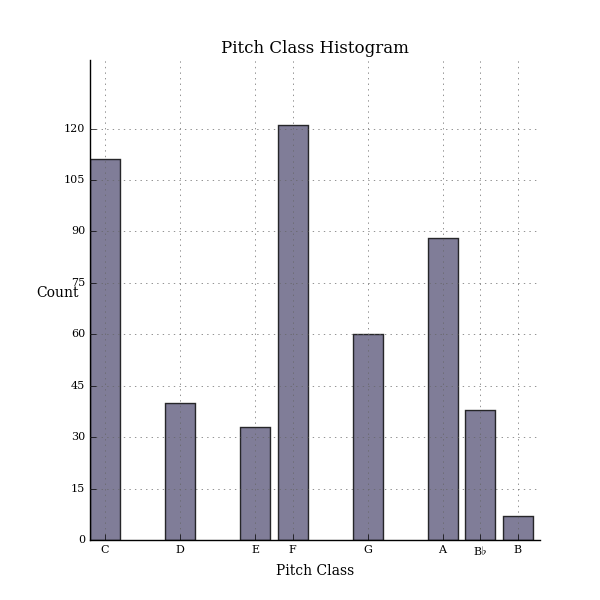
\includegraphics[scale=0.71]{../analysis/bwv1/pitch-class.png}
  \caption{Histograma de \emph{pitch-class} do BWV1.6. \textbf{Fonte}: autor utilizando Music21.}
    \label{fig:pitch-class-bwv1-histogram}
\end{figure}
\section{Resultados}\label{sec:resultados}

Comandos foram utilizados para a estruturação de ``Corais'', pequenas peças didáticas de, por colagem de materiais da bachianos, recorte por técnica \emph{glitch}\footnote{Aplicação de recortes indeterminados  sobre um material pré existente.}, e readequações de discurso harmônico pós-tonal. Resultados foram possíveis com a implementação da a opção \verb|--CAC| ou \verb|-C|, como no código abaixo. No entanto esta é apenas uma \emph{flag} indicativa que um material será reconfigurado. Inclui, até o momento, a \emph{flag} \verb|--glitch| ou \verb|-g|, que recorta o material fornecido.

\begin{listing}
\begin{minted}[linenos,frame=leftline,fontsize=\footnotesize]{python}
./main.py --show --CAC --composer bach --index bwv1 --glitch 2
./main.py -S -C -c bach -i bwv1 -g 2
\end{minted}
\end{listing}

\subsection{BWV1}\label{sec:bwv1}

Experimentamos uma aplicação de erros no sexto movimento de \emph{Wie schün leucht der Morgenstern} (Cantata para a festa da Anunciação, 1725, ver figura \ref{fig:bwv1_frag}). Foi gerado um conjunto de simultanóides apresentados na figura \ref{fig:bwv1_extract}.

\begin{figure}[h]
  \centering
  {%
\parindent 0pt
\noindent
\ifx\preLilyPondExample \undefined
\else
  \expandafter\preLilyPondExample
\fi
\def\lilypondbook{}%
\input{../analysis/bwv1/2a/lily-0aa3d7a2-systems.tex}
\ifx\postLilyPondExample \undefined
\else
  \expandafter\postLilyPondExample
\fi
}

  \caption{Fragmento do sexto movimento do BWV1. \textbf{Fonte}: \cite{music21_2015}.}
  \label{fig:bwv1_frag}
\end{figure}

\begin{figure}[h]
  \centering
  {%
\parindent 0pt
\noindent
\ifx\preLilyPondExample \undefined
\else
  \expandafter\preLilyPondExample
\fi
\def\lilypondbook{}%
\input{../examples/bwv1/c7/lily-6fc7e149-systems.tex}
\ifx\postLilyPondExample \undefined
\else
  \expandafter\postLilyPondExample
\fi
}

  \caption{Sequência de simultanóides gerados. \textbf{Fonte}: Autor.}
  \label{fig:bwv1_extract}
\end{figure}

 Cada bloco harmônico são notas de um determinado compasso, escolhido ao acaso pelo programa, comprimidas em um único evento. É também  interessante observar uma direcionalidade na tessitura, que vai da região média aos graves, percebida após repetidos usos do comando descrito. 

Detalhamos o método composicional um pouco mais: \begin{itemize}
\item A ordem dos simultanóides foi mantida;
\item Foram escolhidos pontos que delimitam fraseados (silêncio como articulado de frases;);
\item Foi estabelecido que a quantidade de notas em um bloco como fator de tensão;
\item Improvisamos dinâmicas como um dispositivo de ênfase do fraseado harmônico; 
\item Foram modificados um si bemol para si natural no terceiro simultanoide, e um si natural para si bemol no anti penúltimo simultanóide, para criar uma unidade harmônica. 
\item Aplicação de Deslocamento, retardamento ou subtração de elementos de notas.
\end{itemize}

A peça finalizada está na figura \ref{fig:bwv1}.

 \begin{figure}
  \centering
  {%
\parindent 0pt
\noindent
\ifx\preLilyPondExample \undefined
\else
  \expandafter\preLilyPondExample
\fi
\def\lilypondbook{}%
\input{../examples/bwv1/d8/lily-ef199858-systems.tex}
\ifx\postLilyPondExample \undefined
\else
  \expandafter\postLilyPondExample
\fi
}

  \caption{Peça resultante das intervenções. \textbf{Fonte}: autor.}
  \label{fig:bwv1}
\end{figure}

\subsection*{Breve Análise}

As ferramentas analíticas do \emph{m21} auxiliaram na observação de semelhanças e diferenças entre a peça original e a peça variada. Por exemplo, com BWV1 de J.S.Bach, plotamos um histograma na figura \ref{fig:pitch-class-bwv1-histogram}, a partir do comando abaixo

\begin{listing}
\begin{minted}[linenos,frame=leftline,fontsize=\scriptsize]{python}
./m21 --show --composer bach --index bwv1 --plot-histogram-pitch-space
\end{minted}
\label{code:plot}
\end{listing}

Este histograma revela fatos analíticos óbvios, como uma ênfase do \emph{pitch class} 5, Fá, 1$^o$ grau; Dó, 5$^o$ grau, seguido de outras classes, como Lá (3$^o$ grau) e Sol (2$^o$ grau); outros, como Ré (6$^o$ grau) e Si bemol, possuem a mesma quantidade. Por último Mi (7$^o$ grau) e si natural possuem os menores números, talvez como dispositivos cadenciais(quinto compasso, primeiro a terceiro tempo, da figura \ref{fig:bwv1_frag}).

Um histograma também foi gerado para a peça resultante (figura \ref{fig:pitch-class-bwv1-histogram-2}). É possível notar que algumas proporções foram mantidas de maneira aproximada, mesmo com uma quantidade de eventos diminuta. Com a segmentação da peça, um centro tonal ainda é mantido (com os 1$^o$ e 5$^o$ graus em maior número), embora de maneira ambígua (2$^o$, 3$^o$ e 6$^o$ graus possuem a mesma quantidade de aparições).

\begin{figure}[!h]
  \centering
  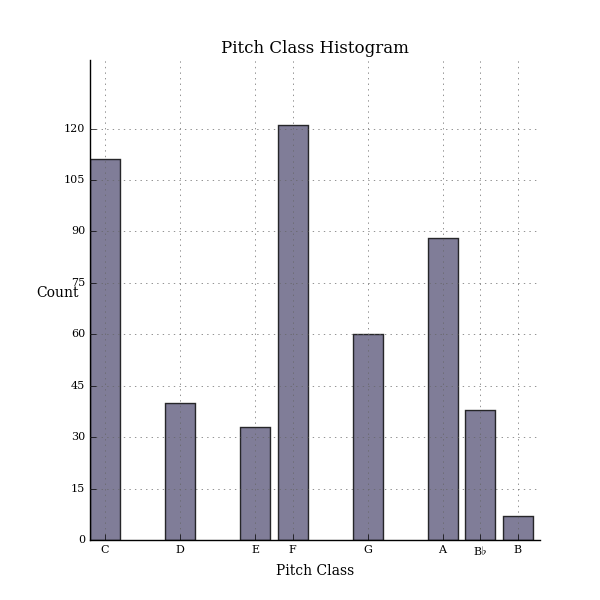
\includegraphics[scale=0.71]{../analysis/bwv1/pitch-class.png}
  \caption{Histograma de \emph{pitch-class} do BWV1. \textbf{Fonte}: Autor}
    \label{fig:pitch-class-bwv1-histogram}
\end{figure}

\begin{figure}[!h]
  \centering
  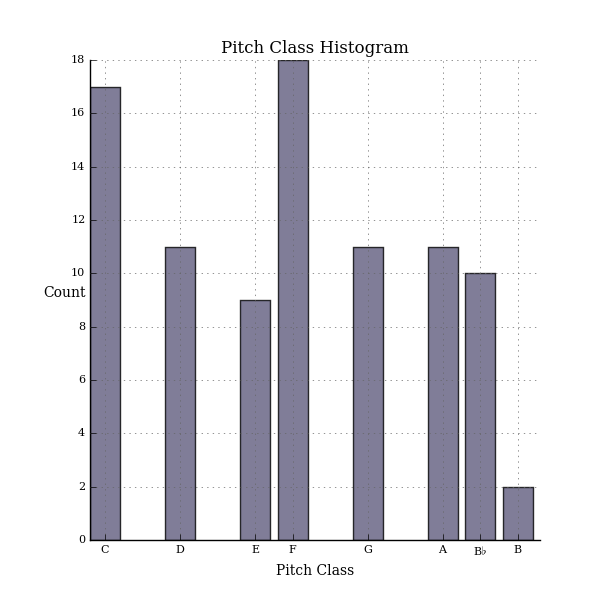
\includegraphics[scale=0.71]{../analysis/bwv1/pitch-class-1.png}
  \caption{Histograma de \emph{pitch-class} da peça Coral \#1. \textbf{Fonte}: Autor}
    \label{fig:pitch-class-bwv1-histogram-2}
\end{figure}



\section{Conclusão}\label{sec:conclusao}

Duas funcionalidades do Music21 foram observadas: Musicologia Assistida por Computador  e Composição Assistida por Computador (CAC).  Da documentação e do corpus do \emph{software}, programei rotinas que lidassem com aquilas tarefas que considerei demasiadamente laboriosas. Para isso proponho comandos que  podem auxiliar em tarefas cotidianas, composicionais ou analíticas. 

Da rotina para composição/análise, cito a busca no corpus, de uma obra específica ou obras pelo nome do compositor. Das rotinas analíticas, enumero \begin{inparaenum}[\itshape a)\upshape]
\item identificação dos graus
\item estruturação intervalar de blocos harmônicos
\item plotamento de histogramas de classes de altura. Das rotinas composicionais, enumerei procedimentos para uma composição por fragmentação (\emph{glitch}):
\item colagem de fragmentos de uma partitura
\item compressão de melodias em blocos harmônicos dos fragmentos resultantes
\item troca de oitavas com as notas deste bloco
\item possível fragmentação do bloco resultante em figuras ou arpejos
\end{inparaenum}Existe adicionalmente um $bug$ que ocorre por fatores lógicos, próprio da atividade de programação realizada, mas ainda não resolvido. Possivelmente o compositor pode lidar com dados nulos. Caso a peça de entrada seja muito grande, pode acontecer do programa não responder. 

Foi observado uma versatilidade de materiais pré-composicionais gerados, bem como a possibilidade de improvisar com estes materiais. O exemplo apresentado na seção \ref{sec:resultados} foi feito em algumas horas. Com isso espero oferecer aos docentes e discentes em composição musical uma ferramenta alternativa para atividades diáticas em processos criativos.

\section{Planos Futuros}

Correção do \emph{bug} e implementação de um novo comando que fragmente várias obras do corpus em um único material pré-composicional (comando \verb|--poop| ou \verb|-p|). Continuação de novas composições para o ciclo.

\section{Agradecimentos}

Ao Guilherme Rafael Soares por apresentar a biblioteca \emph{music 21}. Aos desenvolvedores do \emph{musescore} e \emph{lilypound}. FAPEMIG pelo financiamento da pesquisa.


\clearpage\clearpage
\bibliographystyle{sbc}
\bibliography{article}

\end{document}